\section{电容器的电容}

\subsection{孤立导体的电容}

1.\textbf{孤立导体的电容}:从理论及实验可知,一个孤立导体的电势V与他所带的电荷量q呈线性关系。
$$C=\frac{q}{V}$$

2.他只与导体的大小、形状和周围介质有关。

3.电容是表征导体储电能力的物理量，其物理意义是使导体升高单位电势所需的电荷量，单位：法拉F。

4.孤立导体球半径为R，带电荷为q，则它的电容为$C=\frac{q}{V}=4\pi\varepsilon_{0}R$。

\subsection{电容器的电容}

根据静电屏蔽的原理，用一个封闭的导体壳B将导体A包围起来，使得导体A及导体壳B构成的一对导体系的电势差$V_{A}-V_{B}$不再受到壳外导体的影响，从而维持恒定，这样一个导体系可以称为电容器。

\begin{figure}[h]
	\centering
	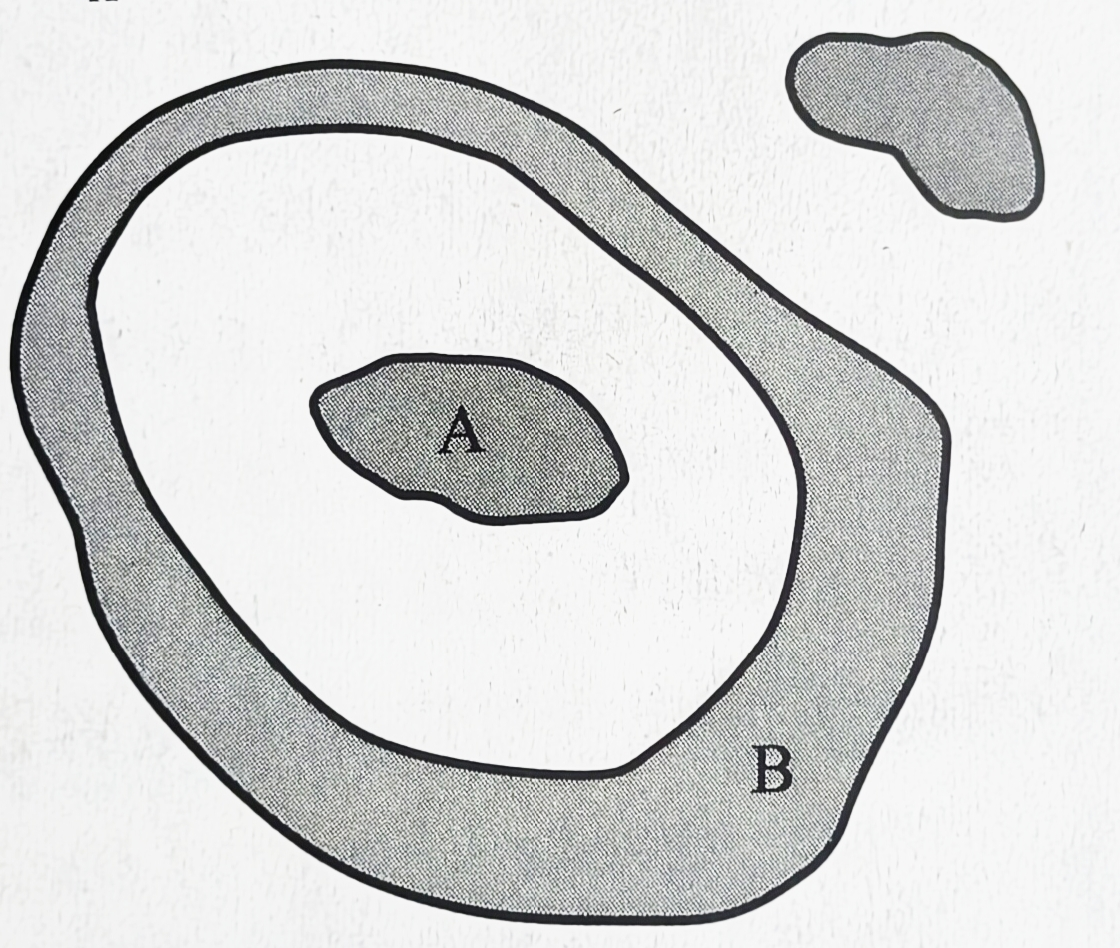
\includegraphics[width=0.3\linewidth]{images/电容器}
	\caption{电容器}
	\label{fig:}
\end{figure}

1.\textbf{电容器的电容}:两导体极板表面上均带有的等量异号电荷q与两极板电势差$\Delta V$的比值。
$$C=\frac{q}{V_{A}-V_{B}}$$

2.实验证明：充有电介质的电容器电容为两板间为真空时的电容$C_{0}$的$\varepsilon_{r}$倍。

其中$\varepsilon_{r}$称为介质的相对电容率或相对介电常量，量纲为1。

\subsection{常见电容器的电容}

\subsubsection{平行板电容器}

两板所带电荷量为q，板间距为d，面积为S，中间充有相对介电常量$\varepsilon_{r} $的电介质，极板的电荷面密度为$\sigma_{0}$。

$$Q=\sigma_{0}S$$

由高斯定理$$D=\sigma_{0}$$

则有$$E=\frac{\sigma_{0}}{\varepsilon_{0}\varepsilon_{r}}$$
$$U=Ed=\int E\mathrm{d}\mathbf{l}$$
$$C=\frac{q}{U}=\frac{\varepsilon_{0}\varepsilon_{r}S}{d}=\varepsilon_{0}\varepsilon_{r}C_{0}$$
\begin{figure}[h]
	\centering
	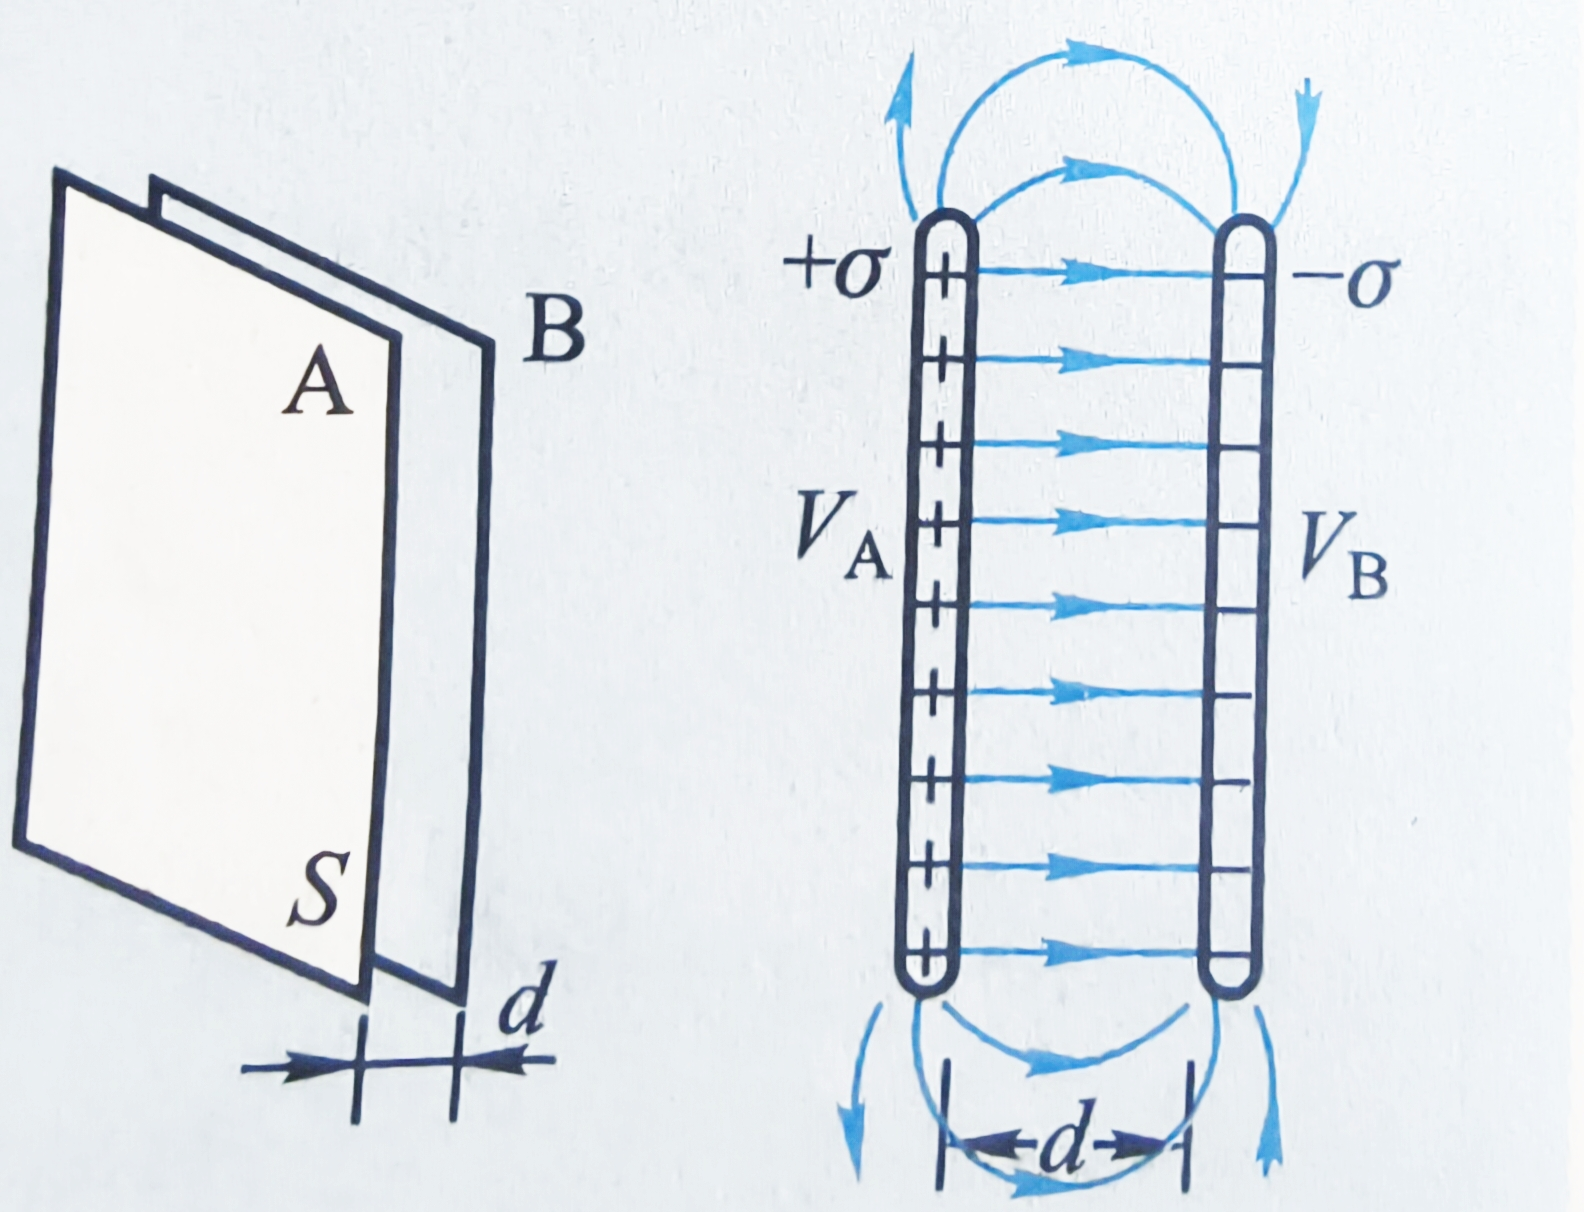
\includegraphics[width=0.4\linewidth]{images/平行板电容器}
	\caption{平行板电容器}
	\label{fig:}
\end{figure}

\subsubsection{同轴圆柱形电容器}

由于两极板距离很近，从两极板中间一点看，可以将其视作无限大带电平面，柱长为L，带电荷量为Q，内半径为$R_{A}$，外半径为$R_{B}$。

设线密度为$\lambda$，$\lambda =\frac{Q}{l}$

取圆柱形高斯面，半径为r,高度为h，则有$$\oint \mathbf{E}\mathrm{d}S=\int_{侧}\mathbf{E}\mathrm{d}S=2\mathbf{E}\pi rh=\frac{\lambda h}{\varepsilon_{0}}$$

求出$$\mathbf{E}=\frac{\lambda}{2\pi\varepsilon_{0}r} $$

则有$$U_{AB}=\int_{R_{A}}^{R_{B}}\mathbf{E}\mathrm{d}r=\int_{R_{A}}^{R_{B}}\frac{\lambda}{2\pi\varepsilon_{0}r}\mathrm{d}r=\frac{\lambda}{2\pi\varepsilon_{0}}\ln\frac{R_{B}}{R_{A}}$$
	
因此$$C=\frac{Q}{U_{AB}}=\frac{2\pi\varepsilon_{0}l}{\ln\frac{R_{B}}{R_{A}}}$$

\begin{figure}[h]
	\centering
	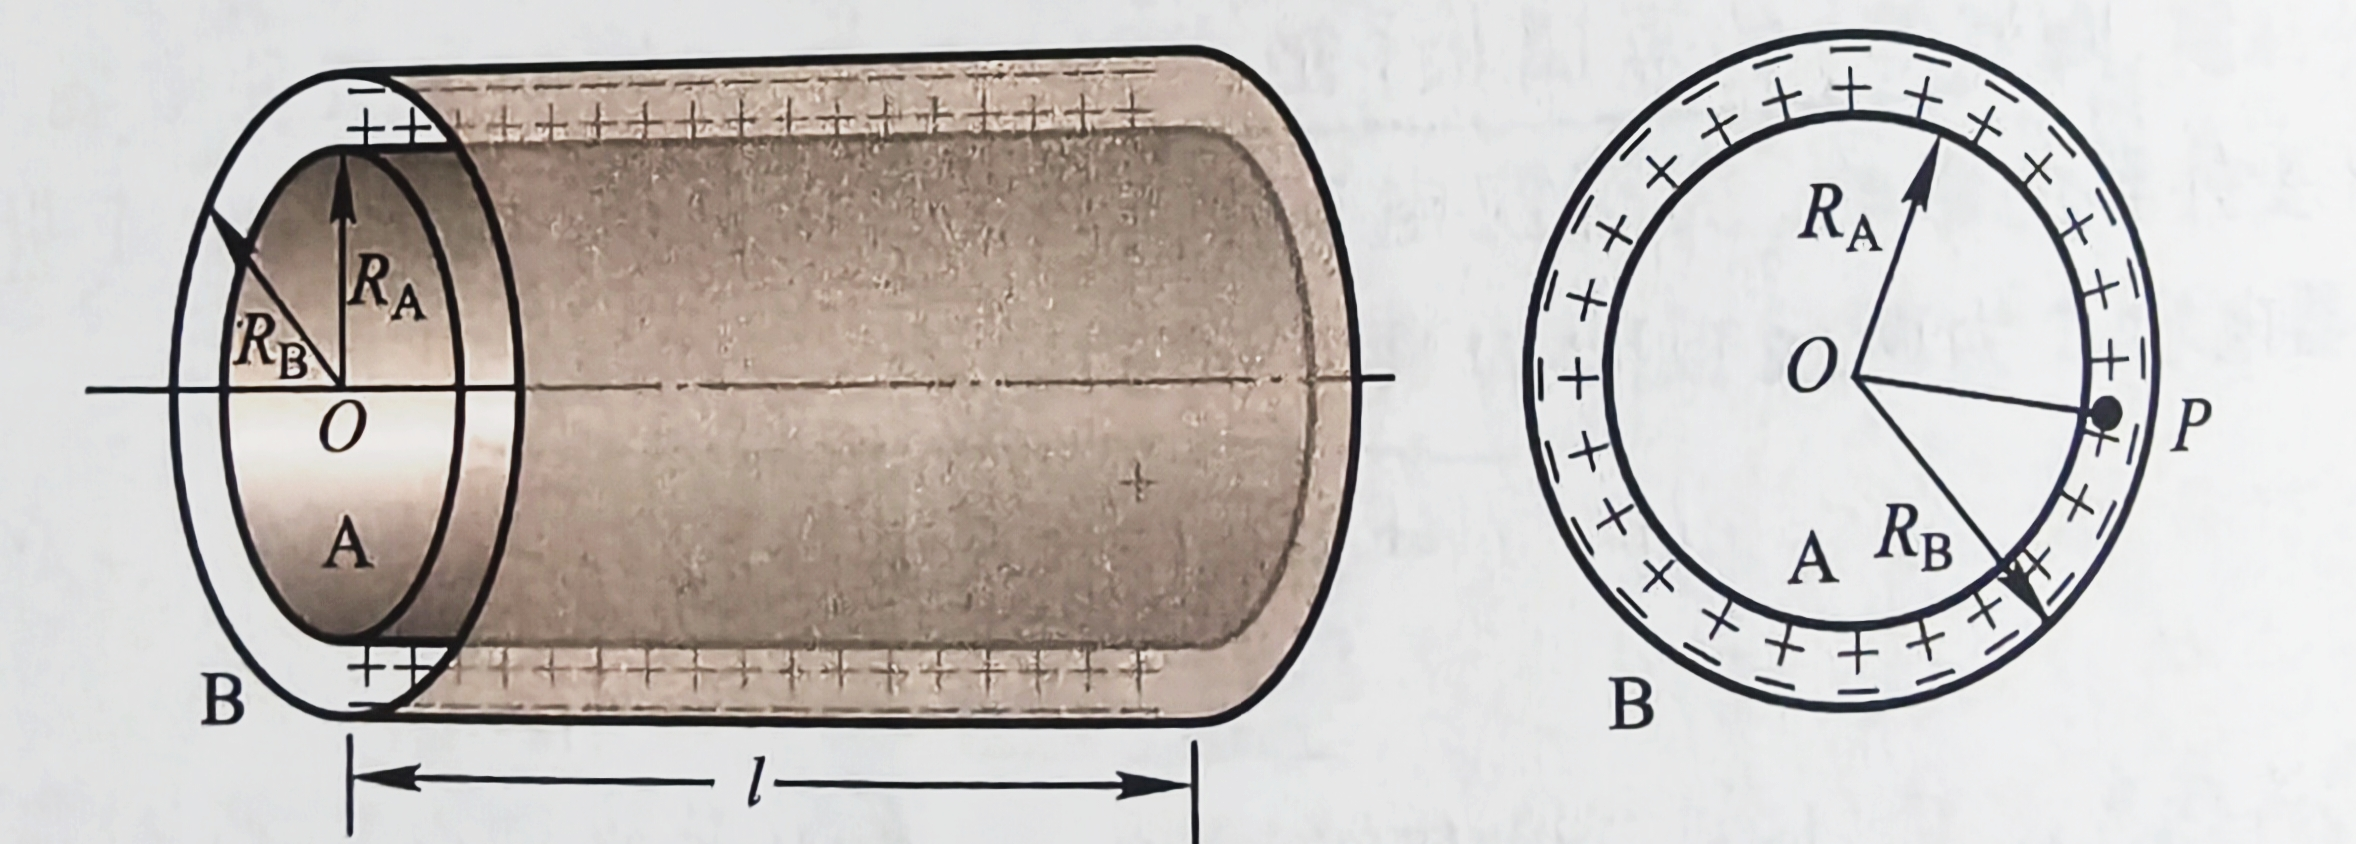
\includegraphics[width=0.5\linewidth]{images/同轴圆柱形电容器}
	\caption{同轴圆柱形电容器}
	\label{fig:}
\end{figure}

\subsubsection{球形电容器}

球形电容器由两个同心的金属球壳组成，内球面半径为$R_{A}$，外球面半径为$R_{B}$，带电荷量为Q。

当$R_{A}<r<R_{B}$时，$$\mathbf{E}=\frac{Q}{4\pi\varepsilon_{0}r^{2}}$$

则$$U_{AB}=V_{A}-V_{B}=\int_{R_{A}}^{R_{B}}\mathbf{E}\mathrm{d}r=\int_{R_{A}}^{R_{B}}\frac{Q}{4\pi\varepsilon_{0}r^{2}}\mathrm{d}r=\frac{Q}{4\pi\varepsilon_{0}}(\frac{1}{R_{A}}-\frac{1}{R_{B}})$$

则$$C=\frac{Q}{U_{AB}}=4\pi\varepsilon_{0}\frac{R_{A}R_{B}}{R_{B}-R_{A}}$$

\begin{figure}[h]
	\centering
	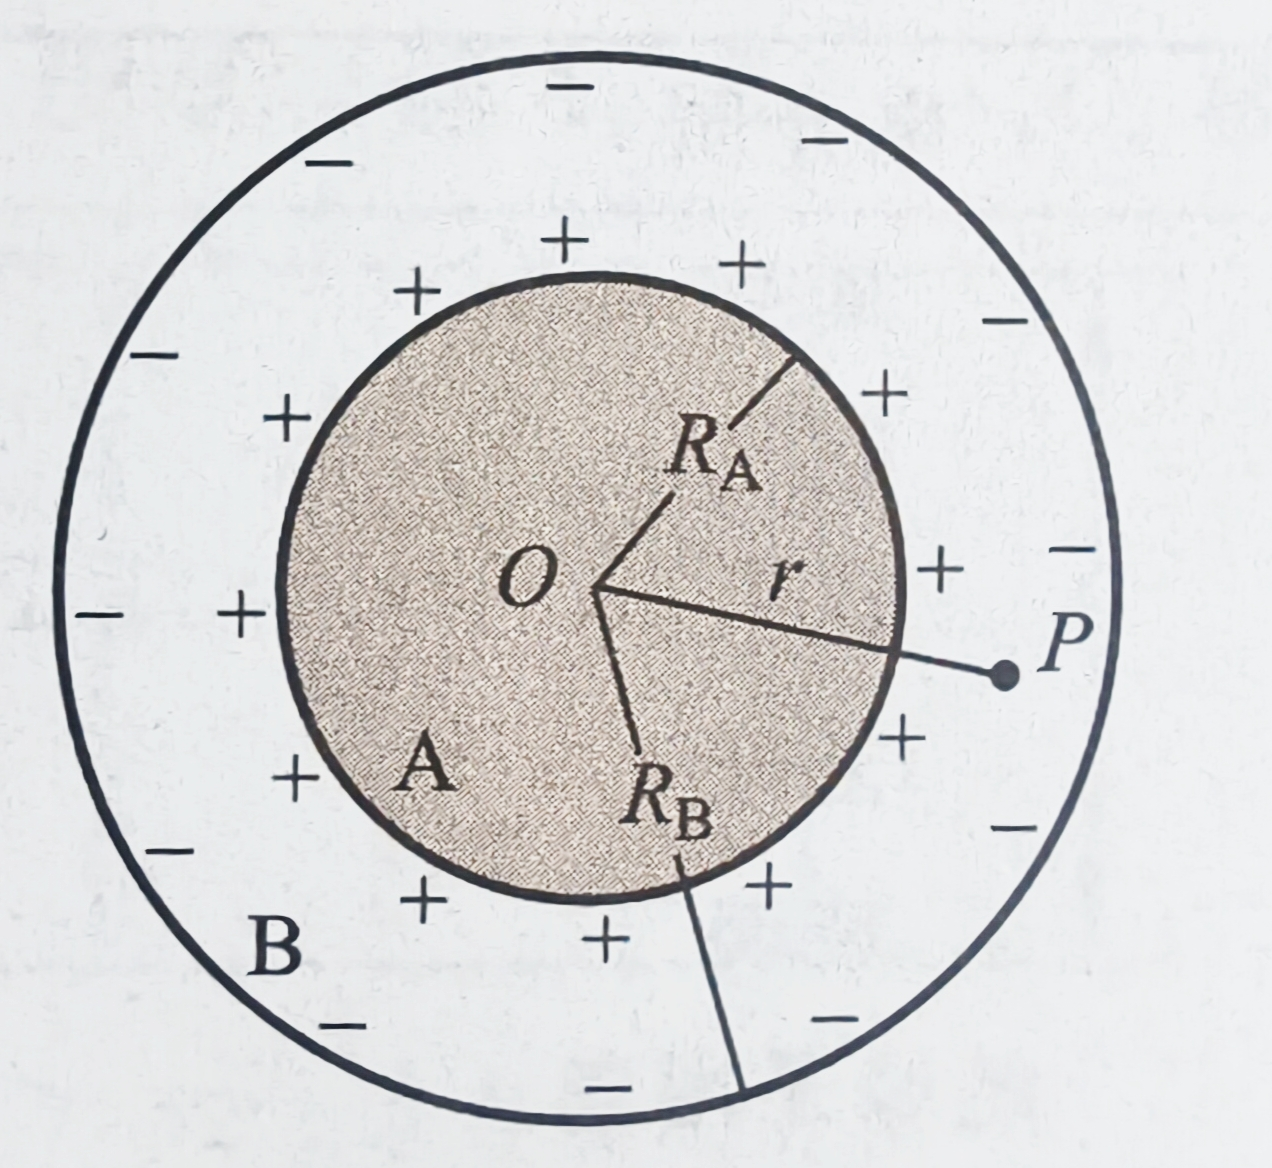
\includegraphics[width=0.4\linewidth]{images/球形电容器}
	\caption{球形电容器}
	\label{fig:}
\end{figure}

\subsection{电容器的串联与并联}

\subsubsection{电容器的串联}

$$C=\frac{Q}{U}=\frac{Q}{U_{1}+U_{2}+U_{3}+......+U_{n}}=\frac{Q}{\frac{Q}{C_{1}}+\frac{Q}{C_{2}}+\frac{Q}{C_{3}}+......+\frac{Q}{C_{n}}}=\frac{1}{\frac{1}{C_{1}}+\frac{1}{C_{2}}+\frac{1}{C_{3}}+......\frac{1}{C_{n}}} $$

\begin{figure}[h]
	\centering
	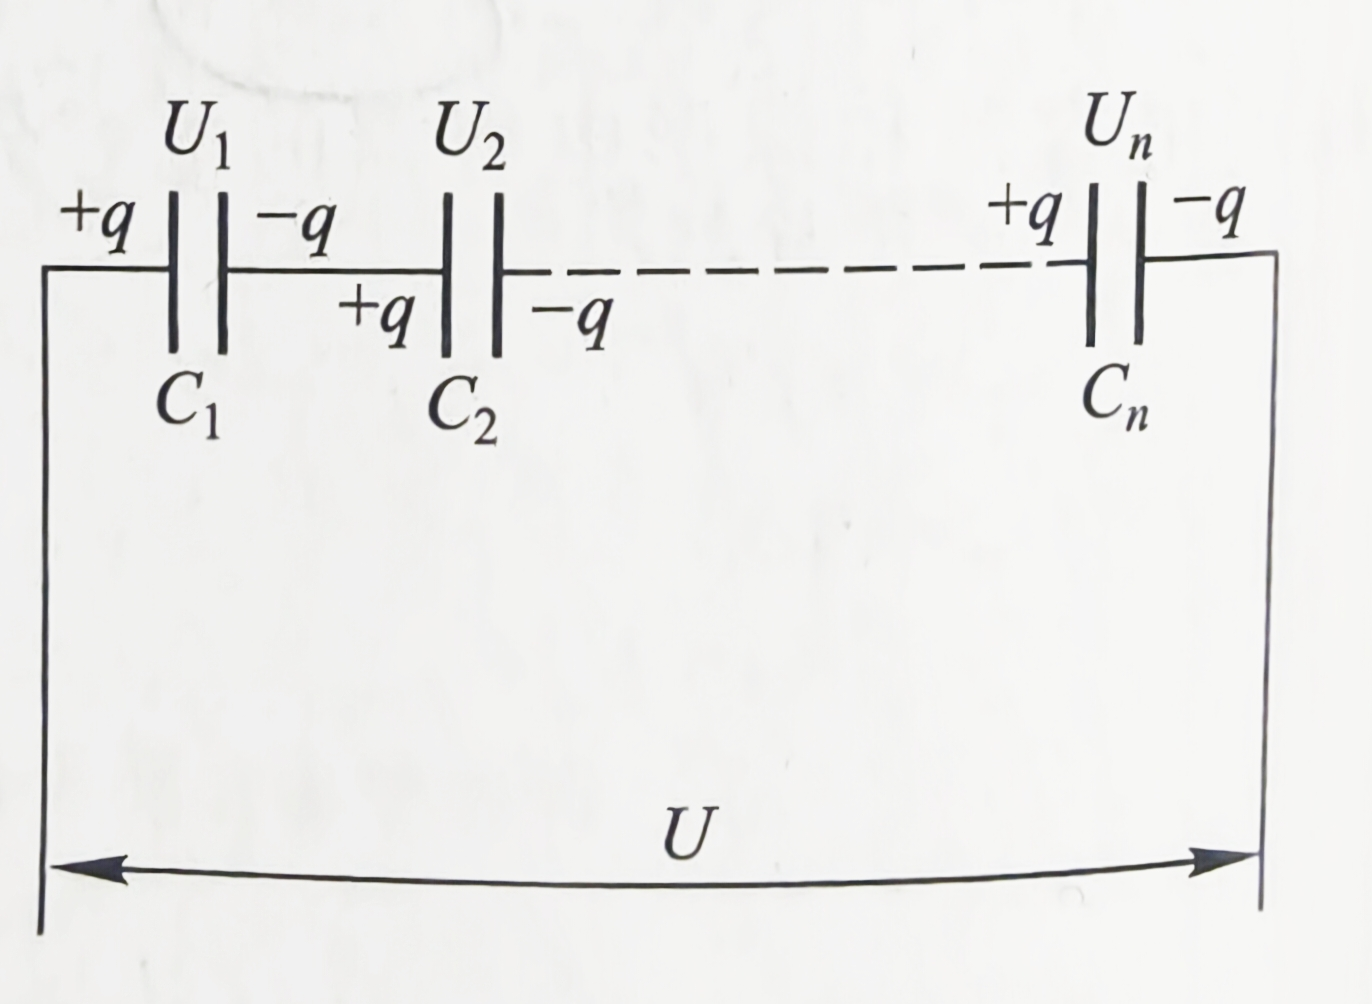
\includegraphics[width=0.4\linewidth]{images/电容器串联}
	\caption{电容器串联}
	\label{fig:}
\end{figure}

\subsubsection{电容器的并联}

$$C=\frac{Q}{U}=\frac{C_{1}U_{1}+C_{2}U_{2}+C_{3}U_{3}+......C_{n}U_{n}}{U} $$

\begin{figure}[h]
	\centering
	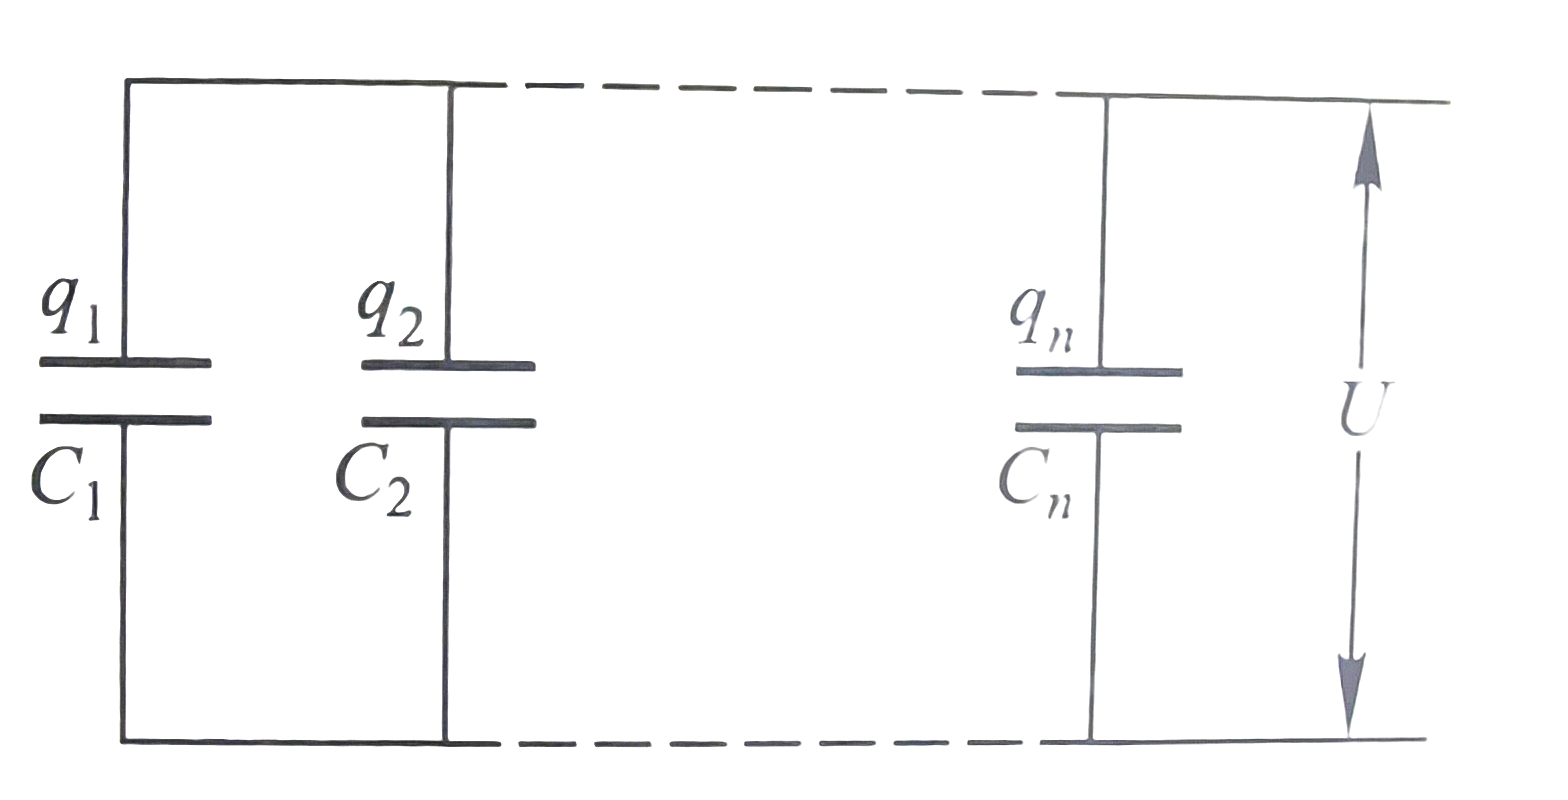
\includegraphics[width=0.5\linewidth]{images/电容器并联}
	\caption{电容器并联}
	\label{fig:}
\end{figure}
